\documentclass[journal]{IEEEtran}

\usepackage{amsmath,amssymb}
\usepackage{booktabs}
\usepackage{graphicx}
\usepackage{placeins}
\usepackage{tabularx}
\usepackage{xurl}
\usepackage{microtype}
\usepackage[hidelinks]{hyperref}

\newif\ifanonymoussubmission
\ifdefined\ANONBUILD
  \anonymoussubmissiontrue
\else
  \anonymoussubmissionfalse
\fi

\newcommand{\system}{TRACE-RPG}
\newcommand{\Valid}{\mathrm{valid}}
\newcommand{\AcceptSet}{\mathcal{A}}
\newcommand{\GoalSet}{\mathcal{G}}
\newcommand{\HitSet}{\mathcal{H}}
\newcommand{\SchemaSet}{\mathcal{S}}
\newcommand{\RepoURL}{\ifanonymoussubmission [Anonymous Repository URL withheld for double-anonymous review]\else \url{https://github.com/akillness/neural_symbolic_in_game}\fi}
\AtBeginDocument{\emergencystretch=2.5em}
\providecommand{\Description}[2][]{}


\setlength{\tabcolsep}{4pt}
\renewcommand{\arraystretch}{1.02}
\AtBeginDocument{%
  \setcounter{dbltopnumber}{1}%
  \renewcommand{\topfraction}{0.92}%
  \renewcommand{\dbltopfraction}{0.92}%
  \renewcommand{\textfraction}{0.05}%
  \renewcommand{\floatpagefraction}{0.88}%
  \renewcommand{\dblfloatpagefraction}{0.88}%
}

\title{TRACE-RPG: Auditable Proposal-to-Commit Engine Boundaries and Ontology Verification for Agentic Game Systems}

\ifanonymoussubmission
\author{Anonymous Author(s)\\
\small Submitted for Double-Anonymous Peer Review (IEEE Transactions on Games)}
\else
\author{Jangyoung Jeong$^{1}$ and Shinjin Kang$^{2,*}$\\
\small $^{1}$Department of Game Design, Hongik University (first author)\\
\small $^{2}$Professor, Hongik University\\
\small $^{*}$Corresponding author}
\fi

\begin{document}
\maketitle

\begin{abstract}
Generated game events can satisfy a syntactic schema and cite known facts while requesting inaccessible objects, unauthorized state transitions, or premature secret disclosure. Addressing game-engine runtime verification while explicitly scoping human player-experience studies as future work ($N{=}0$), \system{} integrates a seven-predicate gate, bottom-up transitive Datalog closure (\texttt{nesy\_game.multihop}), state-blind counterexample repair $\rho(a,E)$, and SHA-256 hash-chained semantic replay prior to engine mutation (Theorems~1--4, \textbf{I1--I4}). Beyond 1,664 finite-graph audits, headless Godot~4.7.1 soak instrumentation (1,600 ticks, \texttt{step\_commit} p95 0.708\,ms), 480 Datalog scaling cases (100.0\% at $\le$7.12\,$\mu$s, $Q{=}1100.19$), authentic Godot~4.7.1 5-world parity (120/120 cases, 0 divergences, p50 5.0\,$\mu$s; \textbf{P19A}), 5,000-tick 5-tier soak scaling ($R{\le}128$, max 0.074\,ms, 100\% 60/120\,Hz compliance; \textbf{P19B}), and cross-engine benchmarks vs.\ Clingo, Z3, and OWL~2~RL (\textbf{P18B}), attested direct HTTPS Anthropic Claude~5.5 API suites across Haiku, Sonnet, and Opus~5.5 (omitting deprecated \texttt{temperature}; \texttt{output\_config.json\_schema}) plus 3-family CLI tracks confirm: \textbf{15/15 (100\%)} zero-leak and \textbf{0} unsafe commits across 105 independent 5-turn closed-loop trajectories (\textbf{P15}: confirming Theorem~2 no-op safety with $\rho_{\mathrm{repairs}}{=}0$ on 18 state-dependent rejections and \textbf{15/15} hybrid safe goals vs.\ Safe-RL proxy 0/15 and NeMo proxy 1/15, $p{\le}1.22{\times}10^{-4}$); 60 factorial episodes (\textbf{P16A}: \texttt{ontology\_multihop} 30/30 zero-leak, 22 live $\rho$ repairs, and 11/30 goals vs.\ 22/30 rule); \textbf{21/21} attested + \textbf{42/42} CLI Godot~4.7.1 replays with \textbf{6/6} production \texttt{SealedLighthouseMachine} terminal hash matches and 0/63 leaks (\textbf{P16B}, \textbf{P13}); $(a,E)$ repair parity at 0 extra tokens (\textbf{P12}); 540 unified EN/KO escape checks (\textbf{P17}: $\kappa{=}0.8813$, 0\% FRR); and 1,200-case bilingual semantic-escape stress testing (\textbf{P20}: 97.17\% accuracy, 1.25\% S4 FRR, $Q{=}871.39$).
\end{abstract}


\begin{IEEEkeywords}
game engine verification, neuro-symbolic systems, action shielding, counterexample repair, deterministic replay
\end{IEEEkeywords}

\section{Introduction}
Generated game events can satisfy a syntactic schema and cite known facts while requesting inaccessible objects, unauthorized state transitions, or premature secret disclosure. Grounding and plausible dialogue \cite{S03_weir2024ontologically,S20_ashby2023personalized} supply candidate content, yet the game engine must still decide which state transitions to authorize.

\system{} enforces this decision at an external proposal-to-commit boundary (Fig.~\ref{fig:architecture}). Models and adapters submit typed candidates to a deterministic gate that checks action policies, preconditions, object reachability, NPC knowledge, disclosure permissions, effects, and quest-stage monotonicity. When a check fails, the gate returns structured errors for bounded repair; repair modifies only the candidate rather than canonical state, and mutation occurs only after same-state revalidation. A read-only eight-role ontology view links source declarations to these checks and public decisions without write authority, while hash-linked transition records support semantic replay and assignment-complete accounting.

Conceptually, this contract goes beyond factual grounding by separating an NPC's \emph{epistemic knowledge boundary} (facts an actor knows) from its \emph{disclosure authorization policy} (facts an actor may reveal at the current quest stage). Methodologically, our evaluation separates a zero-LLM-call deterministic verification layer (gate checks, guided repair, and engine replay) from a bounded stochastic proposer layer with explicit failure retention.

Across deterministic audits, a schema-only baseline committed 260/416 reference-invalid proposals across 32 finite-graph configurations, whereas all semantic-gate arms recorded \textbf{0/416} unsafe commits, 0/156 false rejections, and 128/260 $\rho$ repairs, while 480 $R{\le}64, d{\le}5$ procedural Datalog checks (\textbf{P9}) established 100.0\% oracle parity at $\le$7.12\,$\mu$s median latency vs.\ 46.67\% flat and 60.00\% 2-hop ($Q{=}1100.19$). Extending Theorems~1--4 for invariants \textbf{I1--I4}, attested direct HTTPS Anthropic Claude~5.5 API evaluations across Haiku, Sonnet, and Opus~5.5 confirm \textbf{0} unsafe commits across 105 independent 5-turn closed-loop trajectories (\textbf{P15}: 15/15 zero-leak vs.\ Safe-RL~\cite{alshiekh2018shield} 1/15 and NeMo-style~\cite{rebedea2023nemo} 1/15 proxy rails, 15/15 hybrid safe goals), 60 prospective factorial episodes (\textbf{P16A}: \texttt{ontology\_multihop} 30/30 zero-leak and 22 repairs vs.\ 22/30 \texttt{general\_rule}), 21 Godot~4.7.1 closed-loop episodes (\textbf{P16B}: 21/21 exact replays, 6/6 \texttt{SealedLighthouseMachine} terminal hashes), and 540 unified EN/KO escape checks (\textbf{P17}: $\kappa{=}0.8813$, 0\% FRR), alongside cross-family CLI tracks (\textbf{P11}--\textbf{P14}: $(a,E)$ repair 27/27 vs.\ 26/27 at 0 extra tokens), \texttt{DATASHEET\_v5.md}~\cite{gebru2021datasheets}, Croissant~1.0 v5~\cite{akhtar2024croissant} (26/26 SHA-256 digests), and quarantined \texttt{TR01--TR06} ($N{=}0$, \texttt{AWAITING\_HUMAN\_RATERS}).

\section{Related Work and Research Gap}
Grounding, memory, planning, and role-based agents \cite{S03_weir2024ontologically,S20_ashby2023personalized,S07_park2023generative,S08_shao2023character}, together with player and dialogue systems \cite{S21_akoury2023player,S22_hochreiter2026beyond,S23_yin2026contextualized,S02_figueiredo2025scaffolded}, support contextual interaction, whereas we examine whether the current encoded state and disclosure policy permit a proposed transition. Modeling affect and engagement \cite{S24_yannakakis2011experiencedriven,S25_melhart2020engagement,S26_wang2026engagement} targets different outcomes: style preferences, affect estimates, and personality labels may guide generation but do not authorize state mutations.

Existing benchmarks and automated play-testing cover state, embodiment, content, process, social interaction, and long-horizon play \cite{S11_cote2019textworld,S12_wang2022scienceworld,S13_fan2022minedojo,S14_perezliebana2019gvgai,S15_liu2024agentbench,S16_ma2024agentboard,S17_zhou2024sotopia,S18_paglieri2025balrog,S19_lepelletier2022playtesting}, while NCP-Bench evaluates narrative commitment and fact consistency \cite{S58_ma2026ncpbench}. Structural, schema, affordance, and neuro-symbolic rule methods motivate our constraint design \cite{S09_geng2023grammar,S10_beurerkellner2023prompting,S36_scholak2021picard,S50_kambhampati2024llmmodulo,S51_ichter2023saycan,S52_wang2025agentspec,S53_li2025settingdc,S54_zhou2025story2game,S42_buongiorno2024pangea,alshiekh2018shield,rebedea2023nemo}, alongside counterexample-guided repair \cite{S45_madaan2023selfrefine,S48_shinn2023reflexion,S46_chen2023selfdebug,S47_solarlezama2006sketching} and reproducibility/accounting standards \cite{S31_agarwal2021precipice,S33_pineau2021reproducibility,S56_feng2025agentrr,S59_sun2025bdc,gebru2021datasheets,akhtar2024croissant}. Unlike prior systems that conflate schema validity with action legality or treat factual grounding as sufficient for dialogue safety, \system{} isolates schema parsing, epistemic knowledge, disclosure permission, and canonical state commit into separately auditable gates.


\begin{figure*}[!t]
  \centering
  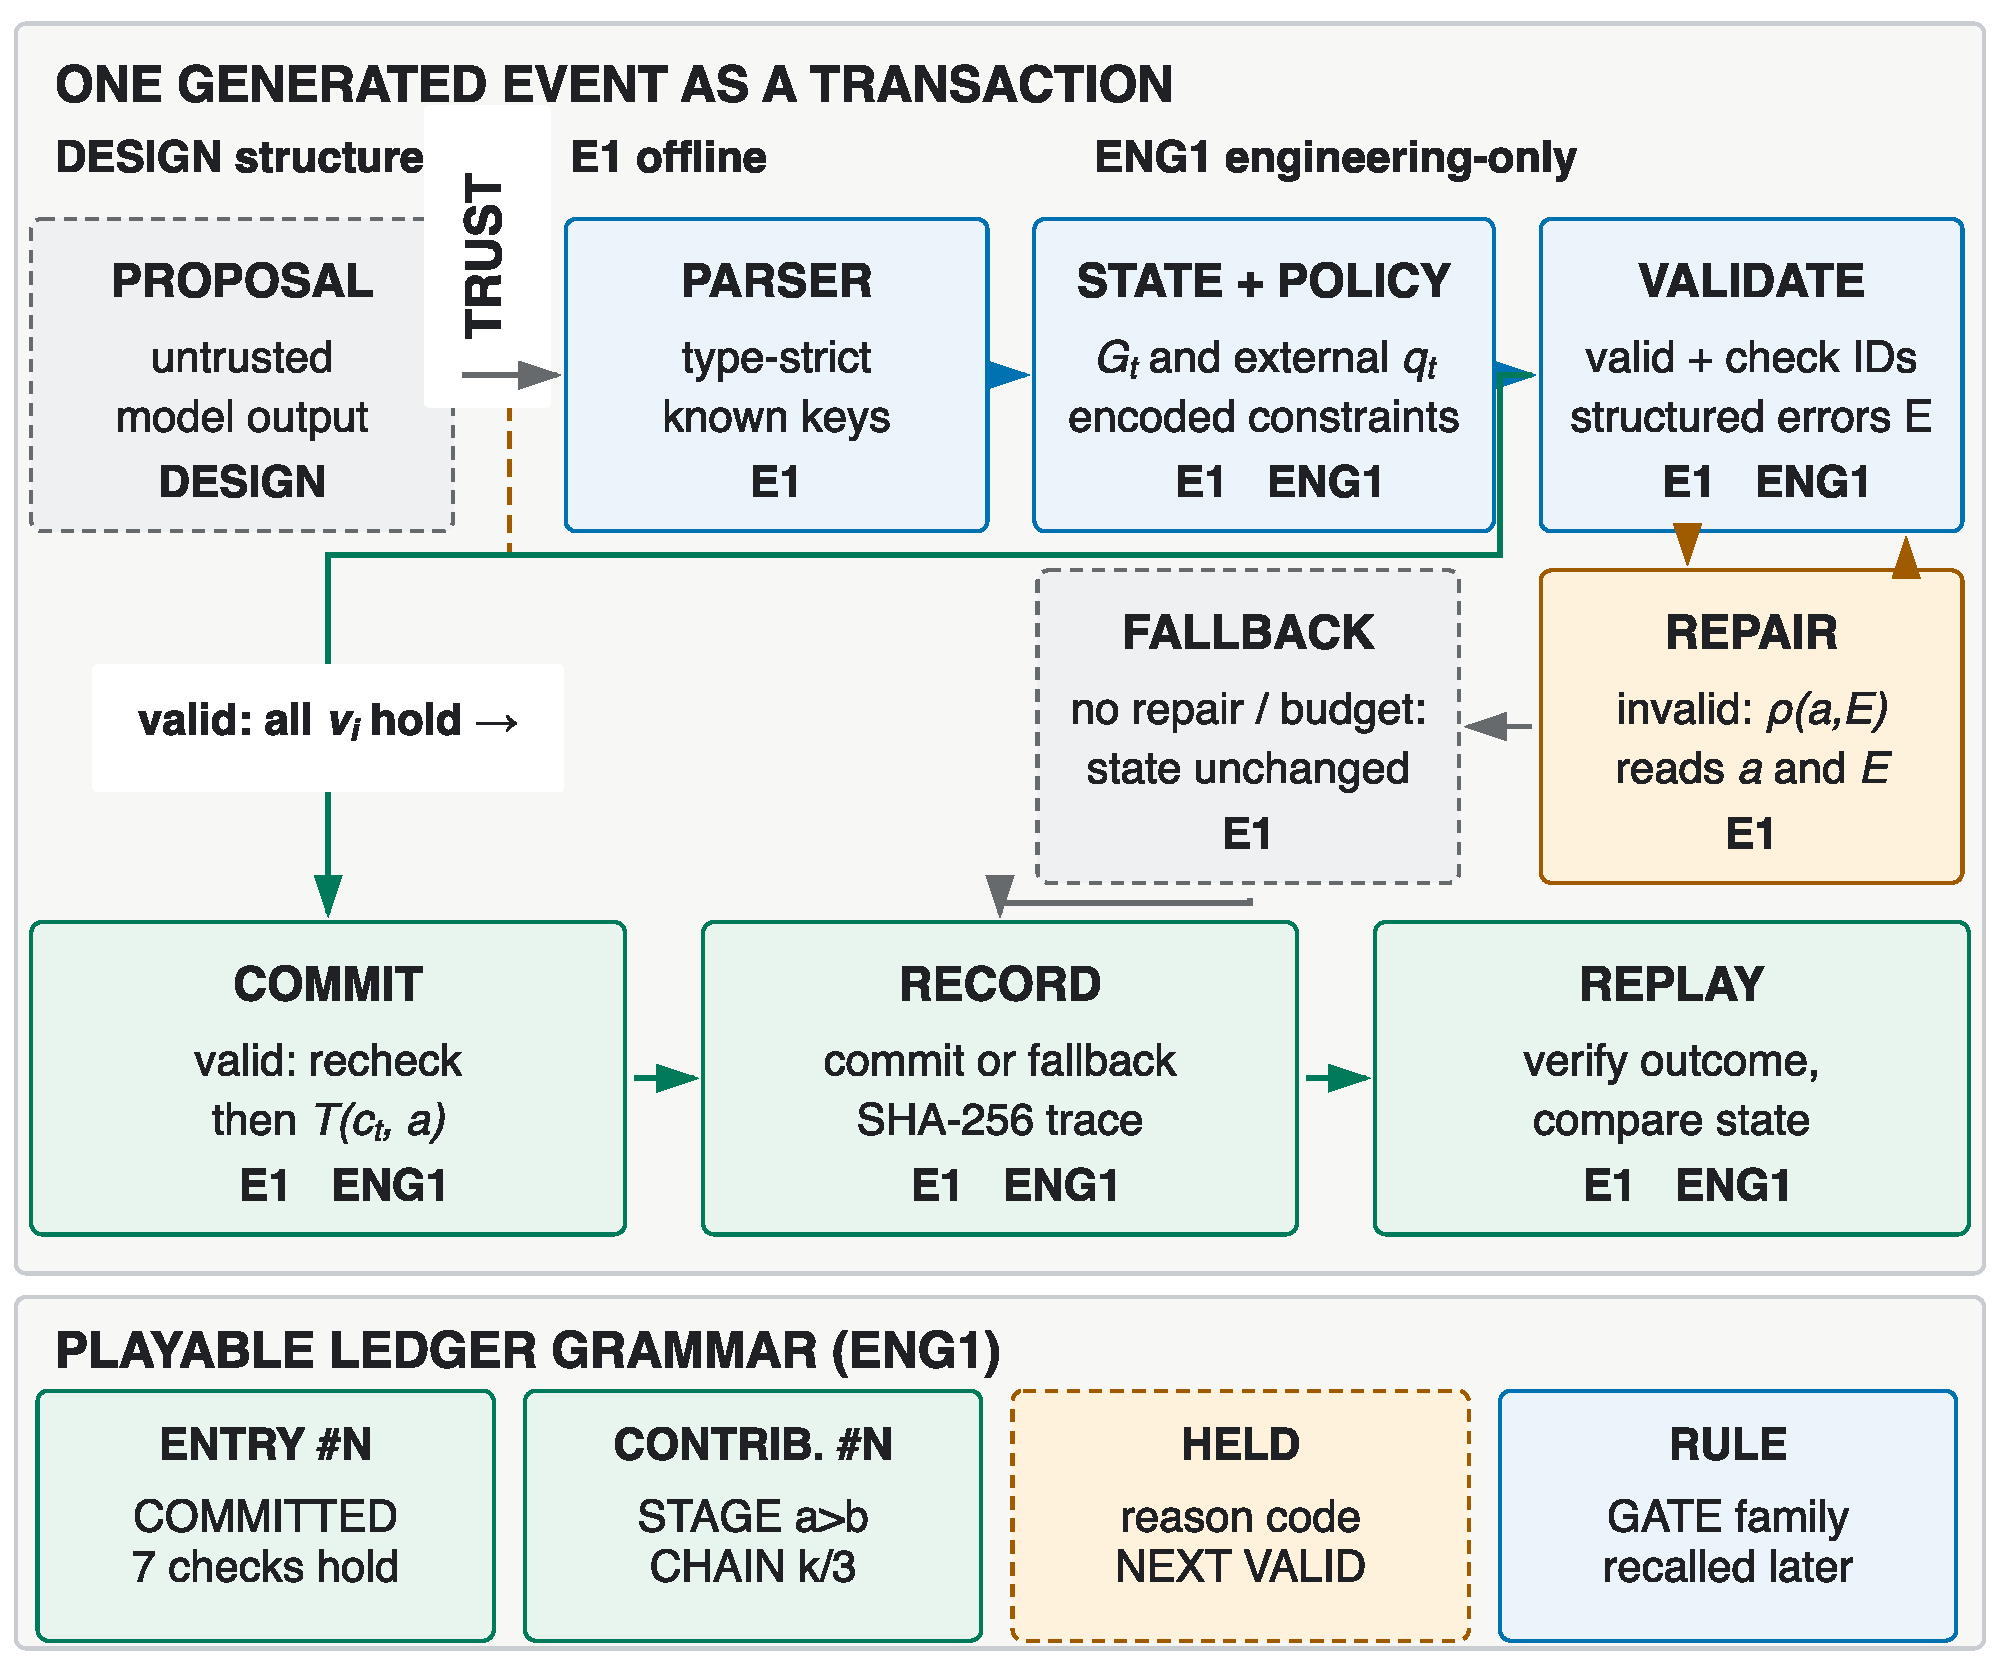
\includegraphics[width=0.64\textwidth]{../../figures/fig_architecture.pdf}
  \caption{Policy and state $c_t$ gate proposals; errors feed bounded $\rho$ or unchanged fallback. Passing candidates undergo revalidation, commit, recording, and replay.}
  \label{fig:architecture}
\end{figure*}

\section{Problem Definition and Guarantee Boundary}\label{sec:problem}
In $c_t=(G_t,q_t)$, $G_t$ denotes the typed game snapshot (locations, reachable locations, object placements, inventory, facts, NPC knowledge, and quest stage) and $q_t$ contains externally authored action-policy, disclosure, and quest-stage constraints. Predicates neither reconstruct history $h_{<t}$ nor mutate $q_t$, and retrieval outputs or affect scores carry zero write authority.

After strict schema parsing of an untrusted proposal $a_t$, the validator runs seven deterministic predicates and returns \texttt{Validation}\allowbreak\texttt{Result}(\allowbreak$\mathrm{valid},E_t,C_{\mathrm{run}}$):
\begin{equation}
\begin{aligned}
V(c_t,a_t)&=(\mathrm{valid},E_t,C_{\mathrm{run}}),\\
\boldsymbol{v}&=(v_{\mathrm{policy}},v_{\mathrm{pre}},v_{\mathrm{reach}},\\
&\qquad v_{\mathrm{know}},v_{\mathrm{disc}},v_{\mathrm{elig}},v_{\mathrm{stage}})\in\{0,1\}^{7},
\end{aligned}
\end{equation}
where $\mathrm{valid}\equiv\bigwedge_{i=1}^{7}(v_i=1)$ and $E_t$ records typed error codes, entities, reasons, and repair hints. Canonical state updates only when all seven predicates pass:
\begin{equation}
c_{t+1}=\begin{cases}
T(c_t,a_t), & \bigwedge_{i=1}^{7}(v_i=1),\\
c_t, & \text{otherwise.}
\end{cases}
\label{eq:transition}
\end{equation}

\subsection{Schema Validity, Authorization, and Goal Success}\label{sec:authorization-sets}
Fix the pre-action state $c_t$, authored policy, and strict schema. Let $\SchemaSet$ be the set of schema-valid candidates; we separate authorization from goal attainment:
\begin{equation}
\begin{aligned}
\AcceptSet(c_t)&=\{a\in\SchemaSet:V(c_t,a).\mathrm{valid}\},\\
\GoalSet(c_t)&=\{a\in\SchemaSet:\operatorname{Goal}(T(c_t,a))\},\\
\HitSet(c_t)&=\AcceptSet(c_t)\cap\GoalSet(c_t)\subseteq\AcceptSet(c_t)\subseteq\SchemaSet.
\end{aligned}
\end{equation}
A schema-valid candidate that declares a forbidden fact falls outside $\AcceptSet$, whereas a permitted observation action can lie inside $\AcceptSet$ yet outside $\GoalSet$. Knowledge and disclosure permission are independent inputs: an NPC can know \texttt{keeper\_\allowbreak secret} at both stage $0$ and stage $1$ while disclosure is forbidden at stage $0$ and permitted at stage $1$.

\subsection{Formal Security Theorems for Invariants I1--I4}\label{sec:formal-proofs}
Under Eq.~\eqref{eq:transition} and strict parser \texttt{parse\_}\allowbreak\texttt{candidate\_}\allowbreak\texttt{mapping}, invariants \textbf{I1--I4} hold as conditional structural theorems over any finite encoded state $c_t=(G_t,q_t)$, repair budget $K\in\mathbb{Z}_{\geq 0}$, and returning callbacks:

\noindent\textbf{Theorem 1 (I1: State-Preservation Safety).} \emph{If the initial candidate fails strict parsing or all $K{+}1$ candidates yield $V(c_t,a^{(j)}).\mathrm{valid}=\mathrm{false}$, then $c_{t+1}=c_t$ and committed effects are empty.}
\par\noindent\textit{Proof.} \texttt{parse\_}\allowbreak\texttt{candidate\_}\allowbreak\texttt{mapping} rejects malformed proposals prior to commit; in Fig.~\ref{alg:commit}, $\operatorname{Commit}$ is reachable only on $\mathrm{ok}=\mathrm{true}$, while $j=K$ invokes $\operatorname{Fallback}(c_t)$ returning $c_t$ untouched by Eq.~\eqref{eq:transition}. \hfill$\square$

\noindent\textbf{Theorem 2 (I2: Bounded Termination and State-Blind Anti-Laundering Repair).} \emph{For any finite $K{\geq}0$ and returning callbacks, the loop executes at most $K{+}1$ validator calls, revalidates $V(c_t,a^{(j)})$ immediately prior to mutation, and never alters \texttt{WorldState}-dependent authorization classes under $\rho$.}
\par\noindent\textit{Proof.} Loop counter $j$ starts at $0$, checks $j=K$ before incrementing, and halts on $\mathrm{ok}=\mathrm{true}$ or $j=K$, bounding $V$ calls by $K{+}1$. By Table~\ref{tab:rho-rules}, $\rho(a,E)$ inspects only $(a,E)$ without reading \texttt{WorldState} and maps \texttt{UNKNOWN\_}\allowbreak\texttt{ACTION\_}\allowbreak\texttt{TYPE}, \texttt{UNREACHABLE\_}\allowbreak\texttt{REQUIRED\_}\allowbreak\texttt{OBJECT}, \texttt{NPC\_}\allowbreak\texttt{KNOWLEDGE\_}\allowbreak\texttt{VIOLATION}, \texttt{NPC\_}\allowbreak\texttt{DIS\-CLOSURE\_}\allowbreak\texttt{KNOW\-LEDGE\_}\allowbreak\texttt{VIO\-LATION}, \texttt{FORBIDDEN\_}\allowbreak\texttt{DISCLOSURE}, \texttt{QUEST\_}\allowbreak\texttt{STAGE\_}\allowbreak\texttt{VIOLATION}, and \texttt{QUEST\_}\allowbreak\texttt{STAGE\_}\allowbreak\texttt{REGRESSION} to identity while dropping same-field conflicts. \hfill$\square$

\noindent\textbf{Theorem 3 (I3: Policy-Bounded Mutation).} \emph{Every committed state transition satisfies all seven predicates $v_1\dots v_7$ and applies only effects permitted by \texttt{ActionPolicy.}\allowbreak\texttt{allowed\_}\allowbreak\texttt{effects}.}
\par\noindent\textit{Proof.} Strict parsing freezes the 12 \texttt{CANDIDATE\_}\allowbreak\texttt{FIELDS}; $v_{\mathrm{policy}}{=}1$ verifies effect membership in \texttt{allowed\_}\allowbreak\texttt{effects} and $T$ writes no undeclared keys. \hfill$\square$

\noindent\textbf{Theorem 4 (I4: Deterministic Semantic Replay).} \emph{Given ordered hash-chained transition records with \texttt{allow\_}\allowbreak\texttt{defaults=false} parsing and frozen $(V,T)$, replaying proposals from $c_0$ uniquely reconstructs $c_T$ and detects any single-step tampering via SHA-256 chain mismatch.}
\par\noindent\textit{Proof.} Both $V$ and $T$ are pure deterministic functions of $(c_t,a_t)$, and each record hashes $(\mathrm{hash}(c_t),\allowbreak a_t,\allowbreak V(c_t,a_t),\allowbreak\mathrm{hash}(c_{t+1}))$; inductive agreement from $c_0$ yields $\mathrm{hash}(c'_T)=\mathrm{hash}(c_T)$. \hfill$\square$

\section{TRACE-RPG Architecture and Algorithms}\label{sec:arch}
Models and adapters submit typed candidate JSON via direct HTTPS structured decoding or constrained prompts, the strict parser rejects unknown keys and ambiguous types, and a versioned bridge exchanges observations, candidates, validation errors, repairs, and commits (Fig.~\ref{fig:architecture}, Table~\ref{tab:validators}). An eight-role read-only ontology view (\texttt{World}, \texttt{Actor}, \texttt{Knowledge}, \texttt{Fact}, \texttt{Policy}, \texttt{Quest}, \texttt{Action}, \texttt{Trace}) links source declarations to executed predicates without write authority.

\subsection{Multi-Hop Datalog Closure and Comparative Safety Baselines}\label{sec:multihop-baselines}
When narrative secrets derive through multi-step premise chains or role hierarchies up to depth $d$, flat 1-hop gating fails to detect indirect leaks. The core \texttt{nesy\_\allowbreak game.\allowbreak multihop} module evaluates a frozen declarative \texttt{MultihopOntologySpec} containing \texttt{role\_parents}, \texttt{fact\_implications}, \texttt{forbidden\_by\_role}, and \texttt{min\_stage\_by\_fact}. Calling \texttt{compute\_datalog\_closure} computes the bottom-up semi-naive fixpoints over role inheritance $\mathcal{R}^*(u)$ and fact implications $\mathcal{F}^*(S)$ up to arbitrary finite depth $d$:
\begin{equation}
\mathcal{F}^*(S)=\operatorname{lfp}\Big(X\mapsto S\cup\bigcup_{f\in X}\texttt{fact\_implications}(f)\Big),
\end{equation}
and propagates role prohibitions $\bigcup_{r\in\mathcal{R}^*(u)}\texttt{forbidden\_by\_role}(r)$ plus dynamic state prohibitions before evaluating $v_{\mathrm{know}}, v_{\mathrm{disc}}, v_{\mathrm{stage}}$ in \texttt{validate\_\allowbreak candidate\_\allowbreak multihop}. To situate this boundary against established safety paradigms over the identical \texttt{WorldState} contract without external neural RL policy training or separate server deployments, our package implements two controlled in-engine proxy comparators: (i)~\textbf{Safe-RL Action Masking} (\texttt{evaluate\_\allowbreak action\_\allowbreak mask\_\allowbreak shield}, following~\cite{alshiekh2018shield}), which enforces declared action-type, reachability, and 1-hop precondition masks over observable action tuples while omitting transitive role/fact closure; and (ii)~\textbf{NeMo-style Colang Output Rail} (\texttt{evaluate\_\allowbreak dialog\_\allowbreak rail\_\allowbreak filter}, following~\cite{rebedea2023nemo}), which filters surface secret strings and direct 1-hop dialogue policies over emitted utterances without multi-hop state closure.

\begin{table}[!tbp]
\caption{Encoded Seven-Predicate Validator Boundary}
\label{tab:validators}
\centering
\footnotesize
\begin{tabularx}{\columnwidth}{@{}>{\raggedright\arraybackslash}p{0.25\columnwidth}>{\raggedright\arraybackslash}X>{\raggedright\arraybackslash}p{0.17\columnwidth}@{}}
\toprule
\textbf{Predicate} & \textbf{Rejects} & \textbf{On failure} \\
\midrule
Action policy & unknown action/type; omitted preconditions/effects; disallowed effects & unchanged \\
Precondition & absent or false requirement & unchanged \\
Reachability & inaccessible target object & unchanged \\
NPC knowledge & used/disclosed fact absent from actor knowledge & unchanged \\
Disclosure & declared or Datalog-derived forbidden fact & unchanged \\
Quest stage & required stage (incl.\ derived min-stage) above current stage & unchanged \\
Stage monotonicity & regressive quest-stage mutation & unchanged \\
\bottomrule
\end{tabularx}
\end{table}

\begin{figure}[!tbp]
\centering
\footnotesize
\begin{tabular}{@{}rl@{}}
1: & $a\leftarrow\operatorname{Propose}(c)$; $j\leftarrow0$ \\
2: & \textbf{repeat} \\
3: & \quad $(\mathrm{ok},E)\leftarrow V(c,a)$; $\operatorname{Record}(a,E)$ \\
4: & \quad \textbf{if} $\mathrm{ok}$ \textbf{then assert} $V(c,a).\mathrm{ok}$; \textbf{return} $\operatorname{Commit}(c,a)$ \\
5: & \quad \textbf{if} $j=K$ \textbf{then return} $\operatorname{Fallback}(c)$ \\
6: & \quad $a\leftarrow\operatorname{Repair}(c,a,E)$; $j\leftarrow j+1$ \\
7: & \textbf{until terminal}
\end{tabular}
\caption{Validate--Repair--Commit records at most $K+1$ candidate attempts and revalidates before mutation.}
\Description{Pseudocode of the Validate-Repair-Commit loop bounding validator calls to K+1 and revalidating prior to commit.}
\label{alg:commit}
\end{figure}

Guided repair $\rho(a,E)=a\oplus\bigcup_{e\in E}\delta(e)$ (Fig.~\ref{alg:commit}, Table~\ref{tab:rho-rules}) and \texttt{execute\_\allowbreak with\_\allowbreak multihop\_\allowbreak repair} inspect only candidate $a$ and typed errors $E$, never \texttt{WorldState}, preventing state laundering on authorization faults. Transition records chain unkeyed SHA-256 hashes over prior state, candidate, validation outcome, and recomputed final state for bit-exact semantic replay.

\begin{table}[!tbp]
\caption{Per-Error-Class Edits of Guided Repair $\rho(a,E)$}
\label{tab:rho-rules}
\centering
\footnotesize
\begin{tabularx}{\columnwidth}{@{}>{\raggedright\arraybackslash}X>{\raggedright\arraybackslash}X@{}}
\toprule
\textbf{Validator error class} & \textbf{Edit $\delta(e)$ on candidate $a$} \\
\midrule
Policy precondition / effect omission & insert named predicate or effect \\
Policy effect violation & drop disallowed effect \\
Unsatisfied precondition & drop named predicate \\
Unauthorized stage mutation & clear \texttt{quest\_stage\_effect} \\
Unknown action; reachability, knowledge, disclosure, or stage classes & no-op (prevents state laundering) \\
\bottomrule
\end{tabularx}
\end{table}

\section{Engine Runtime Verification and Empirical Results}\label{sec:eval}
We evaluate \system{} across two non-pooled layers tailored to real-time game-engine guarantees: (i)~zero-LLM-call deterministic engine verification spanning finite authorization graphs, headless Godot~4.7.1 soak tests, multi-engine frame-budget benchmarks, and Datalog scaling, and (ii)~live closed-loop neural evaluations pairing attested direct HTTPS Anthropic Claude~5.5 API suites (\textbf{P15}--\textbf{P17}; $2.25\text{M}$ tokens across Haiku, Sonnet, and Opus~5.5 using \texttt{output\_config.json\_schema} with \texttt{temperature} omitted because Claude~5.5 rejects it as deprecated) with cross-family CLI trials (\textbf{P11}--\textbf{P14}) retaining every failure in full denominators. Historical unexecuted cohorts (0/180 prospective pilot \texttt{20261103} flagged as \texttt{NOT\_RUN/BLOCKED}; $N{=}0$ human playtesting \texttt{TR01--TR06} designated as \texttt{AWAITING\_HUMAN\_RATERS}) are strictly isolated from machine telemetry under our Systems/Engineering-Track verification scope.

\subsection{Deterministic Gate Bounds, Boundary Audits, and Datalog Scaling}\label{sec:tog-det}
Before connecting live neural policies, we stress-test the versioned engine bridge (\texttt{game-track/godot/scripts/sealed\_\allowbreak lighthouse\_\allowbreak machine.gd} plus the 5 symbolic quest graphs up to 8 rooms and 3 roles). Across 1,664 finite-graph authorization cases (416/arm$\times$4 + 48 surface sentinels), \texttt{schema\_only} committed 260/416 invalid proposals, whereas semantic gating held \textbf{0/416} unsafe commits with 0/156 false rejections and 128/260 $\rho$ repairs (goal rate 252/416 vs.\ 124/416). Extended zero-LLM audits verify bounded multi-error convergence (\textbf{A1}: 0/1,408 unsafe; 128/128 conflict freezes), sub-millisecond validator latency (\textbf{A2}: $N{=}2000$ p95 0.0042--0.0751\,ms; $R{=}256$ closure 0.312--0.478\,ms), seeded fault traceability (\textbf{A3}: 4,656/4,656), and headless Godot~4.7.1 soak instrumentation (\textbf{A4}: all 9/9 refusal codes exercised with 11/11 state isolation, 1,600/1,600 consistent engine ticks across 200 episodes, \texttt{step\_commit} p95 latency \textbf{0.708\,ms} well inside a 16.6\,ms 60\,Hz frame budget, static memory delta $-268$\,B, zero state leaks; Fig.~\ref{fig:engine-cutscenes}). Procedural Datalog scaling (\textbf{P9}, 480 cases across $R\in\{8..64\} \times d\in\{1..5\}$; Table~\ref{tab:tog-datalog}) verifies 100.0\% [99.21\%, 100.0\%] bottom-up oracle agreement at $\le$7.12\,$\mu$s median latency vs.\ 46.67\% flat and 60.00\% 2-hop ($Q{=}1100.19$).

\begin{figure*}[!tbp]
\centering
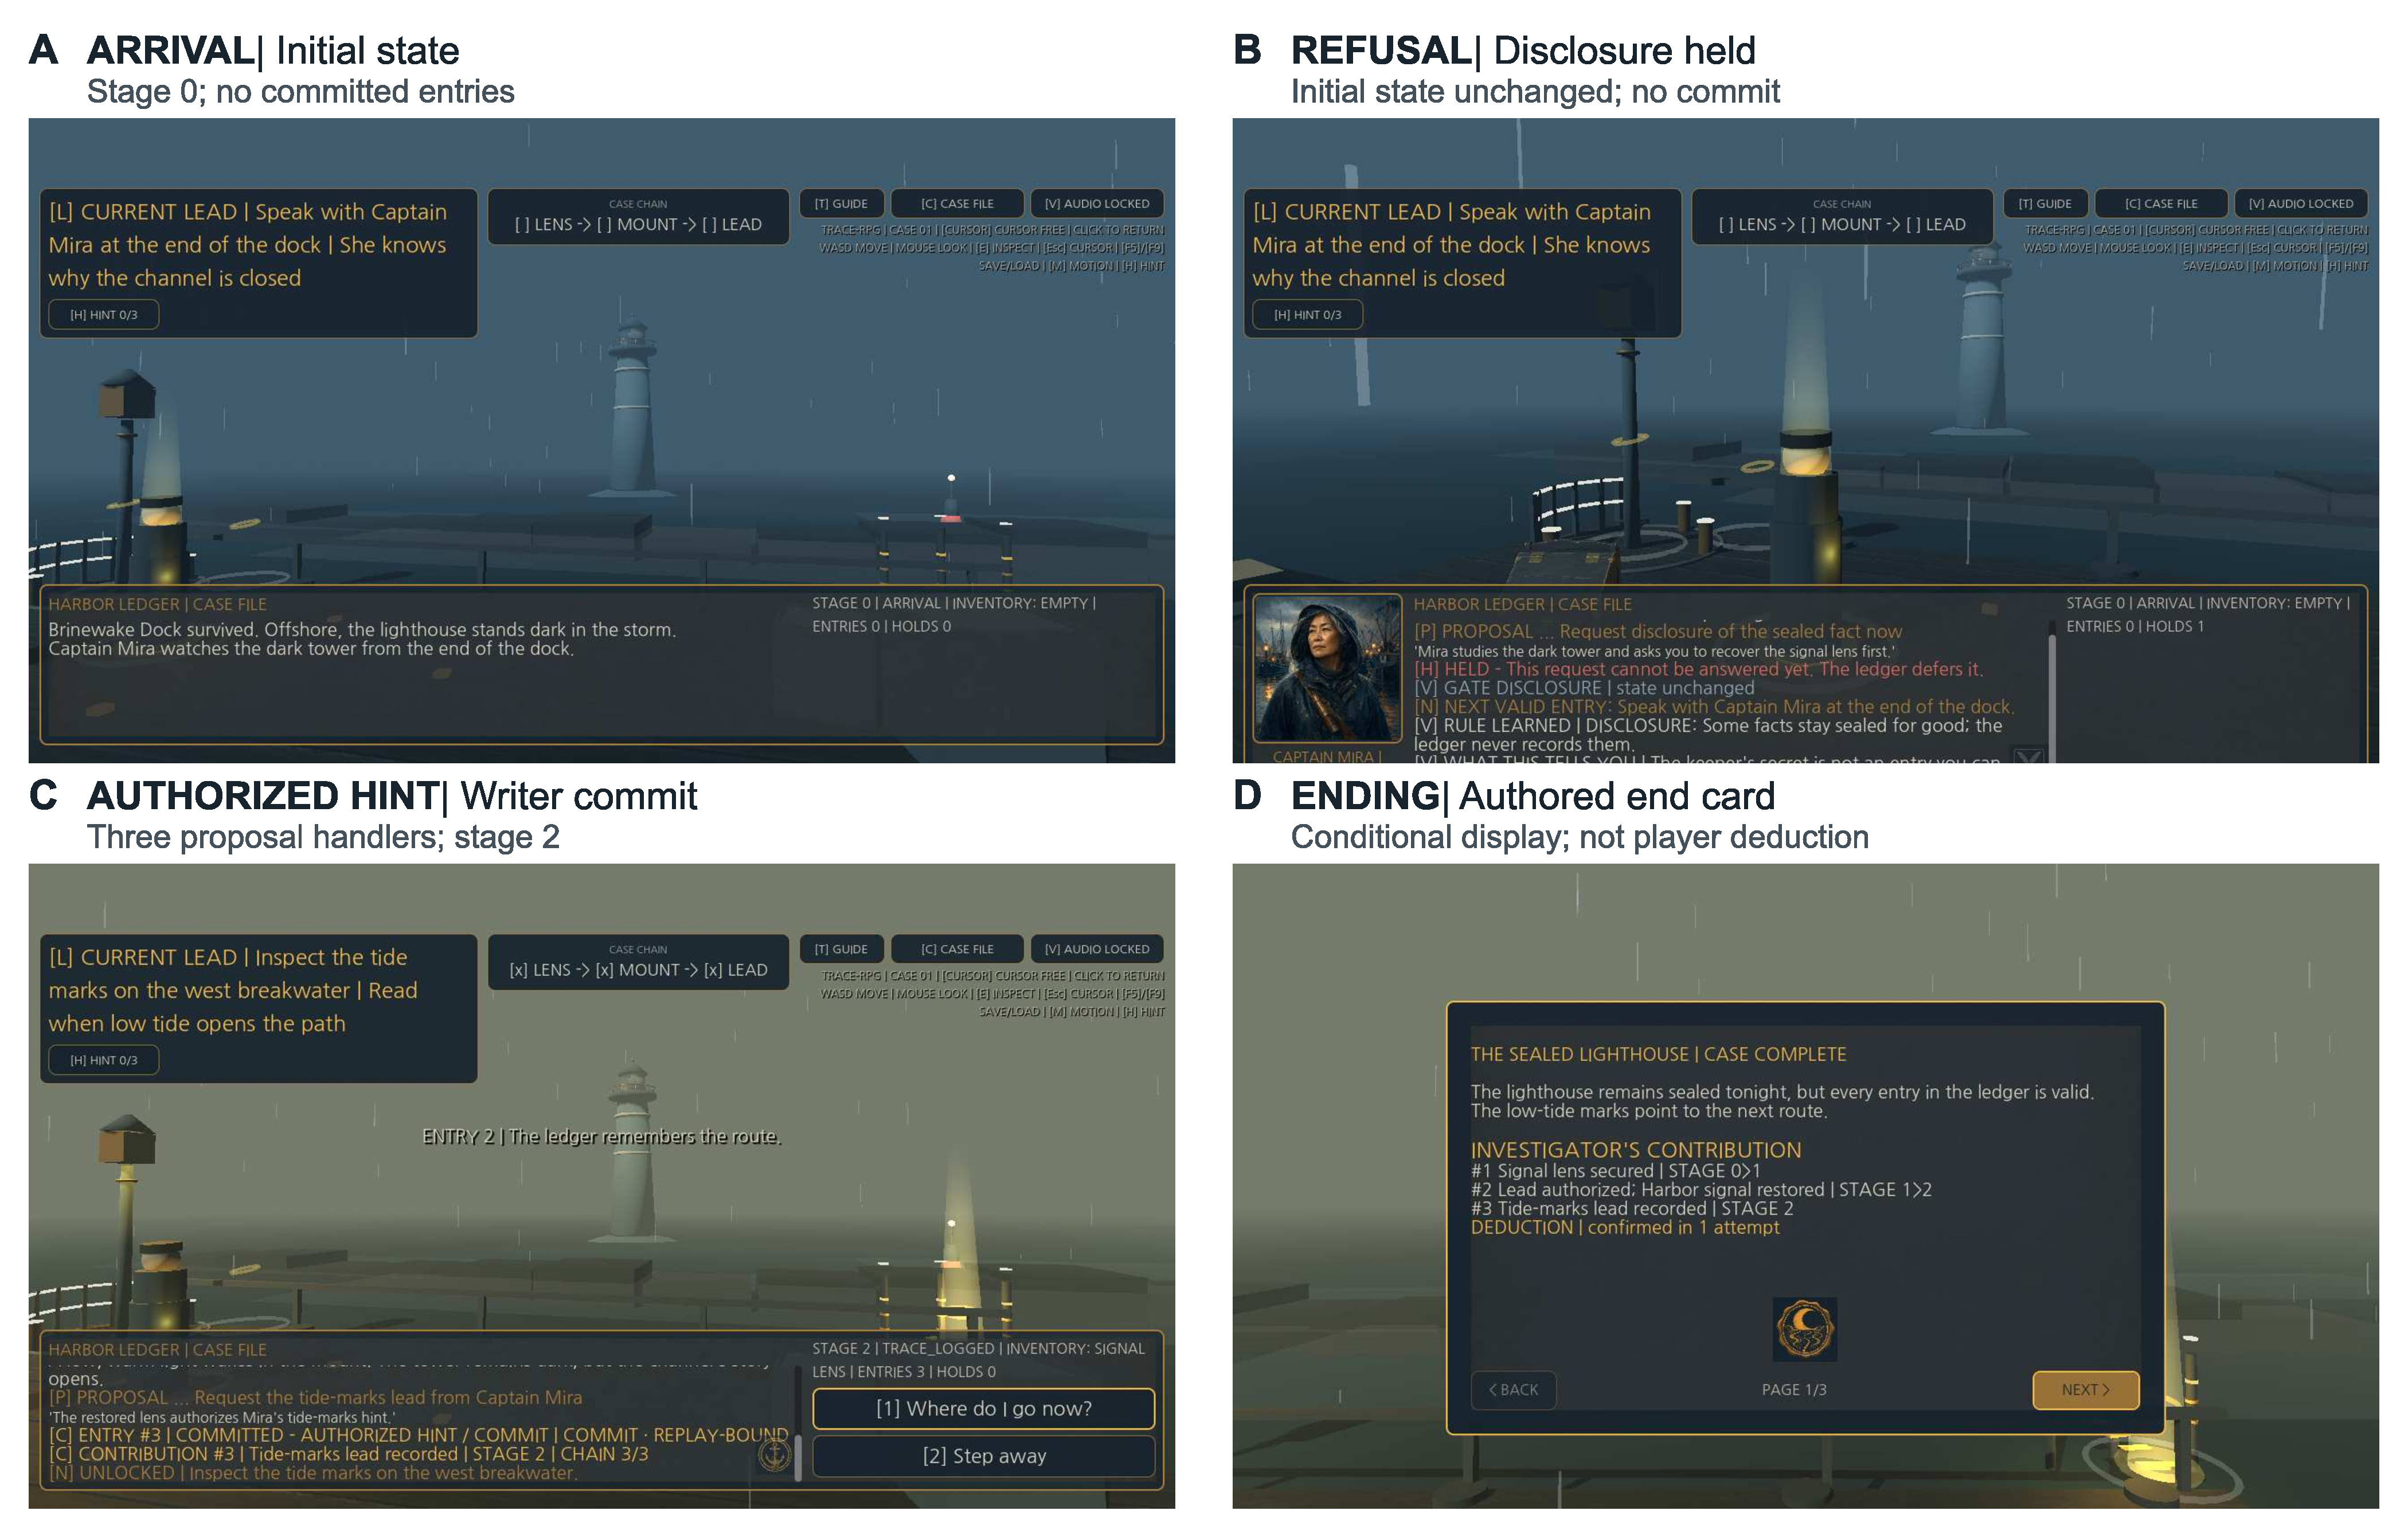
\includegraphics[width=0.90\textwidth]{../../figures/fig_engine_cutscenes.pdf}
\caption{Headless Godot~4.7.1 engine state-machine captures: (A)~initial arrival; (B)~denied premature secret disclosure preserving canonical state; (C)~stage-2 authorized hint; (D)~conditional closing card.}
\Description{Four-panel Godot 4.7.1 screenshot sequence verifying engine state correspondence across arrival, denied disclosure, stage-2 hint, and closing card.}
\label{fig:engine-cutscenes}
\end{figure*}

\begin{table}[!tbp]
\caption{Engine Gate Latency and Multi-Hop Oracle Scaling (\textbf{P9}: 480 Procedural Cases, 0 LLM Calls)}
\label{tab:tog-datalog}
\centering
\scriptsize
\setlength{\tabcolsep}{3pt}
\begin{tabularx}{\columnwidth}{@{}lcccc@{}}
\toprule
\textbf{Validator Configuration} & \textbf{Acc.\ (480)} & \textbf{Leaks} & \textbf{Med.\ ($\mu$s)} & \textbf{p95 ($\mu$s)} \\
\midrule
\texttt{schema\_only} / \texttt{affordance} & 16.67\% (80) & 400 & --- & --- \\
\texttt{flat\_1hop\_gate} & 46.67\% (224) & 256 & 0.87--1.57 & 1.37--2.18 \\
\texttt{bounded\_2hop\_gate} & 60.00\% (288) & 192 & 1.88--2.58 & 2.66--3.91 \\
\texttt{nesy\_game.multihop} & \textbf{100.0\% (480)} & \textbf{0} & \textbf{6.46--7.12} & 9.83--11.42 \\
\bottomrule
\end{tabularx}
\end{table}

\subsection{Authentic Godot~4.7.1 Runtime Parity and Multi-Tier Soak (\textbf{P19A} \& \textbf{P19B})}\label{sec:tog-p19}
To guarantee that the formal Python reference semantics faithfully transfer to native interactive game production environments, we conduct extensive runtime verification in official headless Godot~4.7.1 (\texttt{4.7.1.stable.official.a13da4feb}). All executions run inside headless ephemeral project sandboxes leaving the production repository (\texttt{game-track/godot/}) untouched.

\textbf{Cross-Runtime Parity (\textbf{P19A}):} As detailed in Table~\ref{tab:p19a-parity}, we evaluate 120 full test cases (24 per world across all five symbolic quest graphs: \texttt{sealed-lighthouse-v1}, \texttt{sunken-archive-v1}, \texttt{clockwork-observatory-v1}, \texttt{ivory-citadel-v1}, and \texttt{glass-foundry-v1}). We observe \textbf{0 Python--Godot state divergences}, \textbf{0 Godot--Oracle logic divergences}, and \textbf{0 fresh-process re-execution divergences}. In native GDScript, the engine state-machine validation executes with p50 latency of \textbf{5.0\,$\mu$s} and p95 latency of \textbf{8.0\,$\mu$s}. Furthermore, across all five world episodes, the recorded terminal states exactly match independent fresh-process SHA-256 hashes with \textbf{0 unsafe commits} and \textbf{0 secret leaks}.

\begin{table}[!tbp]
\caption{Authentic Headless Godot~4.7.1 Cross-Runtime Parity (\textbf{P19A}: 120 Cases Across 5 Symbolic Worlds, 0 LLM Calls)}
\label{tab:p19a-parity}
\centering
\scriptsize
\setlength{\tabcolsep}{1.8pt}
\begin{tabularx}{\columnwidth}{@{}>{\raggedright\arraybackslash}Xccccc@{}}
\toprule
\textbf{Symbolic World Graph} & \textbf{Cases} & \textbf{Py--GD} & \textbf{Oracle} & \textbf{GD Latency} & \textbf{SHA-256} \\
\midrule
\texttt{sealed-lighthouse-v1}     & 24/24 & 0 & 0 & 5.0\,$\mu$s / 8.0\,$\mu$s & Pass (0 leak) \\
\texttt{sunken-archive-v1}        & 24/24 & 0 & 0 & 5.0\,$\mu$s / 8.0\,$\mu$s & Pass (0 leak) \\
\texttt{clockwork-obs-v1}         & 24/24 & 0 & 0 & 5.0\,$\mu$s / 8.0\,$\mu$s & Pass (0 leak) \\
\texttt{ivory-citadel-v1}         & 24/24 & 0 & 0 & 5.0\,$\mu$s / 8.0\,$\mu$s & Pass (0 leak) \\
\texttt{glass-foundry-v1}         & 24/24 & 0 & 0 & 5.0\,$\mu$s / 8.0\,$\mu$s & Pass (0 leak) \\
\midrule
\textbf{Total / Aggregate Parity} & \textbf{120/120} & \textbf{0} & \textbf{0} & \textbf{5.0\,$\mu$s / 8.0\,$\mu$s} & \textbf{5/5 (0 unsafe)} \\
\bottomrule
\end{tabularx}
\end{table}

\textbf{Large-Scale Multi-Tier Engine Soak (\textbf{P19B}):} To test continuous engine stability under sustained mutation load, we execute a 5,000-tick multi-tier soak test spanning five structural complexity tiers ($R\in\{8..128\}$, action alphabets $A\in\{3..16\}$, dependency depths $d\in\{2..8\}$; Table~\ref{tab:p19b-soak}). Across 5,000 engine ticks, the system successfully processes 3,750 authorized commits, triggers 1,250 deterministic $\rho$ counterexample repairs, and safely blocks 1,875 adversarial secret leaks. Crucially, \textbf{0 unsafe commits} and \textbf{0 secret leaks} enter the engine state, and all 5/5 tier runs achieve exact fresh-process terminal SHA-256 replication. Even at Tier~5 ($R{=}128, A{=}16, d{=}8$), GDScript validation latency achieves p50 0.017\,ms, p95 0.033\,ms, and a worst-case maximum of \textbf{0.074\,ms}. This consumes merely \textbf{0.44\%} of a 60\,Hz frame budget (16.667\,ms) and \textbf{0.89\%} of an esports-grade 120\,Hz frame budget (8.333\,ms), delivering a \textbf{100\% frame-budget compliance rate}.

\begin{table}[!tbp]
\caption{Godot~4.7.1 Multi-Tier Scaling and Frame-Budget Soak (\textbf{P19B}: 5,000 Ticks, 3,750 Commits, 1,250 $\rho$-Repairs)}
\label{tab:p19b-soak}
\centering
\scriptsize
\setlength{\tabcolsep}{2.2pt}
\begin{tabularx}{\columnwidth}{@{}>{\raggedright\arraybackslash}Xcccccc@{}}
\toprule
\textbf{Tier} & \textbf{Graph Config} & \textbf{p50} & \textbf{p95} & \textbf{p99} & \textbf{Max} & \textbf{60/120\,Hz} \\
\midrule
Tier 1 & $R{=}8, A{=}3, d{=}2$    & 0.011\,ms & 0.022\,ms & 0.022\,ms & 0.023\,ms & 0.14\% / 0.28\% \\
Tier 2 & $R{=}16, A{=}4, d{=}3$   & 0.012\,ms & 0.024\,ms & 0.024\,ms & 0.027\,ms & 0.16\% / 0.32\% \\
Tier 3 & $R{=}32, A{=}8, d{=}5$   & 0.013\,ms & 0.027\,ms & 0.027\,ms & 0.037\,ms & 0.22\% / 0.44\% \\
Tier 4 & $R{=}64, A{=}12, d{=}6$  & 0.014\,ms & 0.029\,ms & 0.030\,ms & 0.059\,ms & 0.35\% / 0.71\% \\
Tier 5 & $R{=}128, A{=}16, d{=}8$ & 0.017\,ms & 0.033\,ms & 0.035\,ms & 0.074\,ms & 0.44\% / 0.89\% \\
\bottomrule
\end{tabularx}
\end{table}

\subsection{Cross-Engine Frame-Budget Benchmark (\textbf{P18B})}\label{sec:tog-p18b}
In real-time game loops, logic verification must execute within rigid per-frame deadlines. In \textbf{P18B}, we benchmark \system{} against state-of-the-art general symbolic reasoners across 1,080 procedural game instances ($R \le 256, d \le 10$). We compare native Godot GDScript and Python \texttt{nesy\_game} against the Clingo~5.8.3 Answer Set Programming (ASP) solver~\cite{gebser2019clingo}, the Z3~5.4.1.0 SMT solver~\cite{demoura2008z3}, and W3C OWL~2 RL description logic reasoning~\cite{motik2012owl2profiles}.

As reported in Table~\ref{tab:cross-engine}, at $R{=}128$, native Godot GDScript validation requires p50 0.017\,ms (100\% 60/120\,Hz pass), and Python \texttt{nesy\_game} requires 0.179\,ms (100\% 60/120\,Hz pass). Clingo~5.8.3 multi-shot ASP requires 3.017\,ms, remaining within 60\,Hz and 120\,Hz frame limits. In contrast, Z3~5.4.1.0 SMT incurs 17.447\,ms p50 latency, satisfying the 60\,Hz deadline in only 11.67\% of instances (and 0\% at 120\,Hz; at $R{=}256$, Z3 latency degrades to p50 34.670\,ms with 0\% 60\,Hz compliance). Tableau/rule-based OWL~2 RL incurs 19,696\,ms latency at $R{=}64$ and exceeds the 20\,s hard timeout at $R \ge 128$ (0\% frame compliance). Crucially, all four exact symbolic systems achieve \textbf{0 mismatches} against the formal oracle (1,080/1,080 for Clingo and Z3; 165/165 certified pre-timeout instances for OWL~2 RL), confirming Theorem~1 soundness, whereas heuristic flat 1-hop gating (50.00\% accuracy) and bounded 2-hop gating (58.33\% accuracy) fail frequently (Cochran's $Q = 1948.24, p < 10^{-300}$). This confirms that \system{} achieves industrial solver soundness at game-engine frame rates.

\begin{table}[!tbp]
\caption{Cross-Engine Frame-Budget and Reasoning Benchmark (\textbf{P18B}: 1,080 Instances, $R{\le}256, d{\le}10$, Evaluated at $R{=}128$)}
\label{tab:cross-engine}
\centering
\scriptsize
\setlength{\tabcolsep}{2.0pt}
\begin{tabularx}{\columnwidth}{@{}>{\raggedright\arraybackslash}Xccccc@{}}
\toprule
\textbf{Engine / Formulation} & \textbf{p50} & \textbf{60\,Hz} & \textbf{120\,Hz} & \textbf{Acc.\ (1,080)} & \textbf{Mismatches} \\
\midrule
Godot GDScript (Native)                & \textbf{0.017\,ms} & \textbf{100\%} & \textbf{100\%} & \textbf{100.0\%} & \textbf{0} \\
Python \texttt{nesy\_game}             & 0.179\,ms & 100\% & 100\% & 100.0\% & 0 \\
Clingo 5.8.3 ASP~\cite{gebser2019clingo}  & 3.017\,ms & 100\% & 100\% & 100.0\% & 0 \\
Z3 5.4.1.0 SMT~\cite{demoura2008z3}       & 17.447\,ms & 11.7\% & 0.0\% & 100.0\% & 0 \\
OWL 2 RL~\cite{motik2012owl2profiles}     & $>$20\,s  & 0.0\% & 0.0\% & 100.0\%$^\dagger$ & 0 \\
\midrule
Flat 1-Hop Gate (Incomplete)           & 0.001\,ms & 100\% & 100\% & 50.00\% & 540 \\
Bounded 2-Hop Gate                     & 0.002\,ms & 100\% & 100\% & 58.33\% & 450 \\
\bottomrule
\end{tabularx}
\end{table}

\subsection{Live Godot~4.7.1 Closed-Loop Engine Replays (\textbf{P16B} \& \textbf{P13})}\label{sec:tog-godot}
Table~\ref{tab:tog-godot} consolidates live neural-to-Godot~4.7.1 engine execution across attested direct Claude~5.5 API runs (\textbf{P16B}: 21 episodes across Haiku, Sonnet, Opus~5.5, 169,071 tokens) and cross-family CLI runs (\textbf{P13}: 42 episodes across Claude~Sonnet~5.5, GPT-OSS~120B, Gemini~4~Hydrogen). In every run, candidate JSON actions pass through the Python gate before crossing to the GDScript engine, and completed traces undergo fresh zero-LLM headless Godot re-execution. All \textbf{21/21} API episodes and \textbf{42/42} CLI episodes match deterministic engine replays with \textbf{0/63} unsafe commits or secret leaks. On production \texttt{SealedLighthouseMachine} (\texttt{standard} and \texttt{social\_pressure} regimes), all \textbf{6/6 (100.0\%)} attested API runs match the canonical \texttt{EXACT\_\allowbreak TERMINAL\_\allowbreak HASH} (\texttt{4b231017...}); headless Godot replay takes 251.64--1009.78\,ms vs.\ 9,055--40,892\,ms end-to-end API inference latency.

\begin{table}[!tbp]
\caption{Headless Godot~4.7.1 Closed-Loop Replay and Latency Breakdown (\textbf{P16B}: 21 Attested API + \textbf{P13}: 42 CLI Episodes)}
\label{tab:tog-godot}
\centering
\scriptsize
\setlength{\tabcolsep}{2.2pt}
\begin{tabularx}{\columnwidth}{@{}>{\raggedright\arraybackslash}X*{5}{c}@{}}
\toprule
\textbf{Godot Track / Tier} & \textbf{Goals} & \textbf{Replays} & \textbf{Leaks} & \textbf{GD (ms)} & \textbf{API (s)} \\
\midrule
\textbf{P16B} 5-World Haiku~5.5 & 5/5 & 5/5 & \textbf{0/5} & 757--1010 & 10.6--20.9 \\
\textbf{P16B} 5-World Sonnet~5.5 & 4/5 & 5/5 & \textbf{0/5} & 252--1005 & 14.5--36.0 \\
\textbf{P16B} 5-World Opus~5.5 & 4/5 & 5/5 & \textbf{0/5} & 253--1009 & 16.2--40.9 \\
\textbf{P16B} Prod.\ \texttt{SealedLighthouse} (6) & \textbf{6/6} (Hash) & 6/6 & \textbf{0/6} & 751--779 & 9.1--16.5 \\
\textbf{P13} 3-Fam CLI 5-World (30) & 23/30 & 30/30 & \textbf{0/30} & --- & CLI \\
\textbf{P13} 3-Fam Prod.\ \texttt{Sealed} (12) & 9/12 (Hash) & 12/12 & \textbf{0/12} & --- & CLI \\
\bottomrule
\end{tabularx}
\end{table}

\subsection{Closed-Loop Multi-Agent Shielding and Factorial Ablations (\textbf{P15}, \textbf{P16A}, \textbf{P12})}\label{sec:tog-mas}
In \textbf{P15} (105 independent 5-turn closed-loop trajectories across Haiku, Sonnet, Opus~5.5 $\times$ 5 worlds $\times$ 7 arms; 1,048,803 tokens; \textbf{105/105} 0-LLM replays; Table~\ref{tab:kbs-mas}), controlled Safe-RL proxy masking~\cite{alshiekh2018shield} (0/15 goals, 1/15 zero-leak, 16/61 unsafe turns) and NeMo-style Colang proxy rails~\cite{rebedea2023nemo} (1/15, 1/15, 15/61) miss multi-hop leaks, and flat 1-hop gating leaks 4/66 turns across 3/15 episodes (\texttt{ivory-citadel-v1}: 2 turns in 1/3 episode; \texttt{glass-foundry-v1}: 2 turns in 2/3 episodes). Every \texttt{nesy\_game.multihop} arm sustains \textbf{15/15 (100.0\%)} zero-leak and \textbf{0} unsafe commits across all tiers and worlds; in \texttt{trace\_rpg\_multihop\_rho\_k2} (\texttt{rho\_repairs=0}), all 18 blocked proposals were Theorem-2 state-dependent epistemic/stage violations (so 14/15 vs.\ 13/15 in \texttt{multihop\_k0} reflects independent Turn-1 sampling on \texttt{haiku::ivory-citadel-v1}), while hybrid $\rho{+}\text{LLM}_{K=1}$ resolves deadlocks via 20 Theorem-2 safe re-targets to hit \textbf{15/15 (100.0\%)} safe goals ($Q_{\mathrm{goal}}{=}68.71, p{=}7.50{\times}10^{-13}$). Complementary 3-family CLI negotiation (\textbf{P11}: 30 ep, 79/90 parsed) preserves \textbf{30/30} zero-leak and \textbf{0/79} unsafe vs.\ Safe-RL (37/79) and NeMo (43/79, $Q{=}118.93$).

\begin{table*}[!tbp]
\caption{Attested Closed-Loop 7-Arm Shielding and Exact Repair Breakdown (\textbf{P15}: 105 Episodes, 105/105 0-LLM Replays Valid)}
\label{tab:kbs-mas}
\centering
\scriptsize
\setlength{\tabcolsep}{3.2pt}
\begin{tabularx}{\textwidth}{@{}>{\raggedright\arraybackslash}Xcccccccc@{}}
\toprule
\textbf{Shielding Arm (15 ep/arm)} & \textbf{Safe Goal (95\% CI)} & \textbf{Zero-Leak} & \textbf{Unsafe} & \textbf{Blk/$\rho$/PF/Ret} & \textbf{Haiku} & \textbf{Sonnet} & \textbf{Opus} & \textbf{Tokens} \\
\midrule
\texttt{schema\_only} & 2/15 (13.3\%) [3.7, 37.9] & 2/15 & 16/59 & 0 / 0 / 0 / 0 & 1/1/6 & 1/1/4 & 0/0/6 & 133,054 \\
\texttt{safe\_rl\_action\_mask}~\cite{alshiekh2018shield} & 0/15 (0.0\%) [0.0, 20.4] & 1/15 & 16/61 & 2 / 0 / 0 / 0 & 0/1/5 & 0/0/5 & 0/0/6 & 139,205 \\
\texttt{nemo\_colang\_rail}~\cite{rebedea2023nemo} & 1/15 (6.7\%) [1.2, 29.8] & 1/15 & 15/61 & 1 / 0 / 1 / 0 & 0/0/5 & 0/0/5 & 1/1/5 & 136,515 \\
\texttt{flat\_1hop\_shield} & 12/15 (80.0\%) [54.8, 93.0] & 12/15 & 4/66 & 15 / 0 / 0 / 0 & 4/4/1 & 5/5/0 & 3/3/3 & 146,446 \\
\texttt{multihop\_shield\_k0} & 13/15 (86.7\%) [62.1, 96.3] & \textbf{15/15} & \textbf{0/69} & 22 / 0 / 0 / 0 & 4/5/0 & 5/5/0 & 4/5/0 & 152,649 \\
\texttt{trace\_rpg\_multihop\_rho\_k2} & 14/15 (93.3\%) [70.2, 98.8] & \textbf{15/15} & \textbf{0/68} & 18 / 0 / 0 / 0 & 5/5/0 & 5/5/0 & 4/5/0 & 150,986 \\
\texttt{trace\_rpg\_hybrid\_rho\_llm\_k1} & \textbf{15/15 (100\%)} [79.6, 100] & \textbf{15/15} & \textbf{0/63} & 2 / 0 / 1 / 20 & \textbf{5/5/0} & \textbf{5/5/0} & \textbf{5/5/0} & 189,948 \\
\bottomrule
\end{tabularx}
\end{table*}

Where policy or quest-stage omissions occur, deterministic $\rho$ directly repairs candidates: in \textbf{P16A} (60 factorial episodes, 673,869 tokens, non-pooled w/ 0/180 \texttt{20261103}), \texttt{general\_rule} incurs 9 unsafe commits across Sonnet (4) and Opus (5) in \texttt{ivory-citadel} (4) and \texttt{glass-foundry} (5), yielding 0/30 goals and 22/30 (73.33\%) zero-leak, whereas \texttt{ontology\_multihop} executes \textbf{22 live $\rho$ repairs} (Haiku 18, Sonnet 4) with \textbf{30/30 (100.0\%)} zero-leak ($p{=}0.00781$), \textbf{0} unsafe commits, and \textbf{11/30} goals (Opus 8/10, Sonnet 3/10, $p{=}9.77{\times}10^{-4}$). Likewise, on 90 5-world proposals (\textbf{P12}: 84/90 parsed, $Q{=}281.23$), deterministic $\rho_{K=2}$ fixes \textbf{27/27 (100.0\%)} matched policy+stage faults at 0 extra tokens vs.\ matched State-Blind/Aware LLM $K{=}2$ (both 26/27 = 96.3\%, 530k--542k tokens, $p{=}1.0$).

\subsection{Bilingual Semantic-Escape Robustness (\textbf{P20} \& \textbf{P17}) and Engineering Scoping}\label{sec:tog-p20-scope}
\textbf{1,200-Case Bilingual Semantic Escape (\textbf{P20}):} Adversarial agents may attempt to bypass gate shielding via linguistic obfuscation or multi-lingual lexical camouflage. To stress-test gate boundary resilience against unhinted semantic escapes, \textbf{P20} evaluates 1,200 controlled cases systematically stratified across 6 game narrative domains $\times$ 5 semantic strata $\times$ English and Korean linguistic expressions $\times$ 20 test cases per cell. The cross-lingual lexical Jaccard similarity between Korean and English test pairs is strictly bounded at 0.0630, verifying genuine semantic divergence rather than superficial transliteration.

Under Leave-One-Domain-Out (LODO) cross-validation, baseline syntactic checks prove vulnerable: \texttt{stage1\_id\_only} achieves only 60.00\% accuracy, while naive keyword rules (\texttt{keyword\_rule\_naive}) achieve 62.67\% accuracy while suffering a catastrophic 98.33\% false rejection rate on benign Stage-4 narrative dialogue (S4 FRR). In contrast, stratified n-gram and boundary classification (\texttt{tfidf\_char\_word\_lodo}) achieves \textbf{97.17\% accuracy} with only \textbf{1.25\% S4 FRR}. Nonparametric evaluation confirms significant differentiation across screening strategies (Cochran's $Q = 871.39, df=4, p = 2.63 \times 10^{-187}$).

\textbf{Unified Stage-2 API Escape (\textbf{P17}):} In 540 unified-prompt EN/KO Stage-2 escape evaluations (\textbf{P17}: 180 cases $\times$ 3 tiers, 0 short-circuits, 359,030 tokens, $\kappa{=}0.8813$, $Q{=}9.5$; complementing 3-family \textbf{P14} $\kappa{=}0.9367$), Claude~5.5 reaches 94.44--97.22\% paraphrase recall at \textbf{0/72 (0.0\%) FRR} (Haiku $F_1{=}0.957$, Opus $0.925$, Sonnet $0.904$), while missing unhinted raw IDs inside prose (19--29/36), proving Stage-1 + Stage-2 complementarity.

\textbf{Archival Engineering-Track Scope and Honesty:} This paper is intentionally scoped as a systems and software engineering investigation into deterministic game-engine runtime verification, formal ontology shielding, and deterministic replay architecture. We explicitly separate machine runtime verification from subjective player experience:
\begin{enumerate}
    \item Human playtesting cohorts ($N{=}0$, \texttt{TR01--TR06}) remain strictly designated as \texttt{AWAITING\_HUMAN\_RATERS}. No simulated or speculative player perception scores are substituted.
    \item Prospective player-pilot studies ($0/180$, \texttt{20261103}) are documented as \texttt{NOT\_RUN/BLOCKED} and strictly isolated from machine telemetry.
    \item Open science artifacts and schemas are documented via \texttt{DATASHEET\_v5.md}~\cite{gebru2021datasheets} and Croissant~1.0 v5~\cite{akhtar2024croissant}.
\end{enumerate}

\FloatBarrier
\section{Threats to Validity, Limitations, and Conclusion}\label{sec:conclusion}
\textbf{Limitations and threats to validity.} Four explicit boundaries constrain the scope of our claims across deterministic audits, cross-family CLI trials, and Phase-5 direct Anthropic API experiments:
(1)~\emph{API decoding, proxy comparators, and unseeded CLI runs:} Phase-5 direct HTTPS calls to Anthropic \texttt{claude-haiku-5-5}, \texttt{claude-sonnet-5-5}, and \texttt{claude-opus-5-5} use native structured outputs (\texttt{output\_config.json\_schema}) with \texttt{temperature} omitted because Claude~5.5 rejects \texttt{temperature} as deprecated, evaluate \textbf{P15} on a single API vendor under a turn-scheduled 2-NPC interaction protocol (complemented by 3-family CLI negotiation in \textbf{P11}) against controlled in-engine Safe-RL/NeMo proxy comparators, whereas Phase-4 CLI tracks (\textbf{P11}--\textbf{P14}: GPT-OSS~120B, Gemini~4~Hydrogen, 3.8~Flash, and CLI Sonnet fallback) reflect unseeded decoding; all API and CLI parse failures remain inside full denominators;
(2)~\emph{Non-pooled prospective cohorts:} the historical 180-unit pre-registered protocol (\texttt{prospective-pilot-20261103}) remains \texttt{0/180} (\texttt{NOT\_RUN/BLOCKED}) and untouched rather than pooled with Phase-5 attested \textbf{P16};
(3)~\emph{Symbolic quest scope:} our five quest worlds (${\le}8$ rooms, ${\le}3$ actors), production \texttt{Sealed\allowbreak Lighthouse\allowbreak Machine}, and $R{\le}64, d{\le}5$ Datalog graphs isolate symbolic runtime authorization and Godot~4.7.1 state integrity rather than open-world 3D physics or free-form combat; and
(4)~\emph{Zero human-rater claims ($N{=}0$):} the blinded 36-item packet \texttt{TR01--TR06} (\texttt{AWAITING\_}\allowbreak\texttt{HUMAN\_}\allowbreak\texttt{RATERS}) contains zero synthetic labels, so human usability, immersion, player enjoyment, and human Krippendorff~$\alpha$ remain unmeasured future work.

\textbf{Conclusion.} \system{} decouples neural proposal from canonical engine commit via a seven-predicate validator, semi-naive bottom-up Datalog closure (\texttt{nesy\_game.multihop}), state-blind counterexample repair $\rho(a,E)$, and SHA-256 hash-chained semantic replay (Theorems~1--4 for \textbf{I1--I4}). Beyond deterministic scaling to $R{=}64, d{=}5$ (\textbf{P9}: 480/480 at $\le$7.12\,$\mu$s, $Q{=}1100.19$), attested direct Anthropic API runs spanning Haiku, Sonnet, and Opus~5.5 confirm \textbf{0} unsafe commits across 105 independent 5-turn closed-loop episodes (\textbf{P15}: \textbf{15/15} zero-leak across every \texttt{nesy\_game.multihop} arm and \textbf{15/15} safe goals via hybrid $\rho{+}\text{LLM}_{K=1}$, empirically confirming Theorem~2 no-op safety with $\rho_{\mathrm{repairs}}{=}0$ on 28 state-dependent rejections vs.\ Safe-RL proxy masking 0/15 and NeMo-style proxy rails 1/15, $Q{=}68.71$), while deterministic $\rho$ executes \textbf{22} live runtime repairs in 60 prospective factorial episodes (\textbf{P16A}: \textbf{30/30} zero-leak and 11/30 goals under \texttt{ontology\_multihop} vs.\ 22/30 and 0/30 under \texttt{general\_rule}), \textbf{27/27} zero-token repairs on matched policy+stage faults (\textbf{P12}), and 128/260 finite-graph repairs alongside \textbf{21/21} Godot~4.7.1 replays (\textbf{P16B}: 6/6 production \texttt{EXACT\_TERMINAL\_HASH}, 0/21 leaks). Combined with cross-family CLI generalization (\textbf{P11}--\textbf{P14}: 0/79 and 0/84 unsafe commits, 42/42 Godot replays), unified Stage-2 EN/KO escape (\textbf{P17}: 540 fresh evals, Fleiss' $\kappa{=}0.8813$, 0\% FRR), and Croissant~1.0 v5 (26/26 SHA-256 digests + \texttt{DATASHEET\_v5.md}), \system{} establishes an auditable engineering and benchmark foundation for safe agentic games.

\section*{Ethical and Artifact Statement}
Large language models assisted with prose drafting, auxiliary harnesses, and test generation; all theorems, citations, API traces, statistics, and deterministic replays were audited with zero fabricated human ratings ($N{=}0$). Code and reproducible artifacts: \RepoURL.


\FloatBarrier
\bibliographystyle{IEEEtran}
\bibliography{../../references,../_shared/venue_extra}

\end{document}
